\chapter{Conditioning Consistency across Context, Memory, and Policy Updates}\label{ch:C17}

MemoryWalker identifies training histories that disagree with actual edited rollout views; October's CODA study examines failures when skills and their consuming policy co-adapt~\cite{j2026memorywalker,feng2026coda}. Together they expose two separate consistency questions: whether a likelihood is conditioned on the right information, and whether a changed component preserves intended behavior. Neither question is settled by preserving archive bytes or database transaction order.

\section{One decision depends on several versions}\label{sec:C17:state}
An agent's behavior depends on more than its model weights. The input view, memory store, retrieval index, tool schemas, harness, authorization, and environment each contribute to the conditional decision. Two runs using the same named model can implement different policies if any of these components changes. Conversely, identical stored text can produce different behavior when a new policy interprets it. Consistency is therefore a relation among components and transitions, not a property conferred by one database.

Define the complete system configuration at a decision boundary as
\begin{equation}
 Z_t=(H_t,\mathcal C_t,M_t,X_t,\theta_t,\delta_t,h_t,\mathcal T_t,A_t,\lambda_t,\nu_t,\alpha_t),
\end{equation}
where $H_t$ is recorded evidence, $\mathcal C_t$ the active view, $M_t$ memory, $X_t$ environment state, $\theta_t$ model parameters, $\delta_t$ deployment decoding, $h_t$ harness behavior, $\mathcal T_t$ tool contracts, $A_t$ trusted authority state, $\lambda_t$ the effect ledger, $\nu_t$ compatibility metadata, and $\alpha_t$ the current authority epoch. Not every component is fully observable, particularly the external environment and proprietary model implementation. A consistency claim must state which components it constrains and which remain outside the guarantee.

Let $g_{\nu,h}$ be the versioned context-assembly map, including selection and serialization. Any random assembly choices are retained as decision evidence or as a materialized view, rather than assumed recoverable from a seed alone. Let $A_t^{\rm vis}$ be the policy-safe projection of authority; the trusted monitor can retain more privileged information. The request is part of $H_t$. The deployed proposal law is
\begin{equation}
 \mathcal C_t=g_{\nu_t,h_t}(H_t,M_t,\mathcal T_t,A_t^{\rm vis}),
 \qquad P(a_t\mid Z_t)=\Pi_{\theta_t,\delta_t,h_t}(a_t\mid\mathcal C_t,\mathcal T_t),
\end{equation}
followed by a current-authority enforcement and execution transition. The law includes the parser and stopping semantics of Chapter~\ref{ch:C02}. Governing implementations remain fixed within a comparison epoch; selecting a versioned skill or editing its runtime input can change state without changing its interpreter. A changed executable resource or model checkpoint requires an explicit configuration transition. Restoring $\nu_t$ cannot restore an expired grant or revise $\lambda_t$ without new effect evidence. This formulation is original synthesis. It makes explicit that assembly and monitoring can change behavior without a weight update. It also identifies why a model-only benchmark cannot certify a complete deployed agent.

Consistency has several meanings. Conditioning consistency preserves what was visible when an action was sampled. Semantic consistency preserves the status and scope of assertions across memory transformations. Transactional consistency governs concurrent reads and writes. Computational consistency governs whether cached states correspond to the input being evaluated. Authority consistency preserves the current allowed-action boundary. These properties interact but are not equivalent; satisfying one should not be described as satisfying all.

The three contracts in Chapter~\ref{ch:C01} provide a common test across those mechanisms. Proposal preservation constrains the distribution produced from a transformed view. Authority nonexpansion constrains the admissible effects, even when proposals change. Effect-state preservation constrains the ledger needed to distinguish pending, committed, and reconciled operations. Conditioning consistency adds a training obligation: an unchanged terminal artifact cannot justify assigning an earlier action a history it never saw. Thus a context edit can preserve authority and effect records while changing proposals, and a perfect behavior replay can still be invalid under revoked authority. The component checks need to identify which contract they establish.

The 2026 context-management literature provides concrete instances. MemoryWalker examines rollout and training views~\cite{j2026memorywalker}; CLM couples editable context with serving behavior~\cite{shao2026context}; HyperSkill changes reusable memory while retaining a task-level retrieved context~\cite{xu2026hyperskill}. Their mechanisms occupy different transitions in $Z_t$. A coherent architecture must specify how those transitions compose rather than assuming that each component's local improvement remains beneficial after integration.


% SCIENTIFIC_FIGURE_C17
Figure~\ref{fig:C17:overview} compares action laws under a fixed deployment and different views of common recorded history.
\begin{figure}[!htbp]
\centering
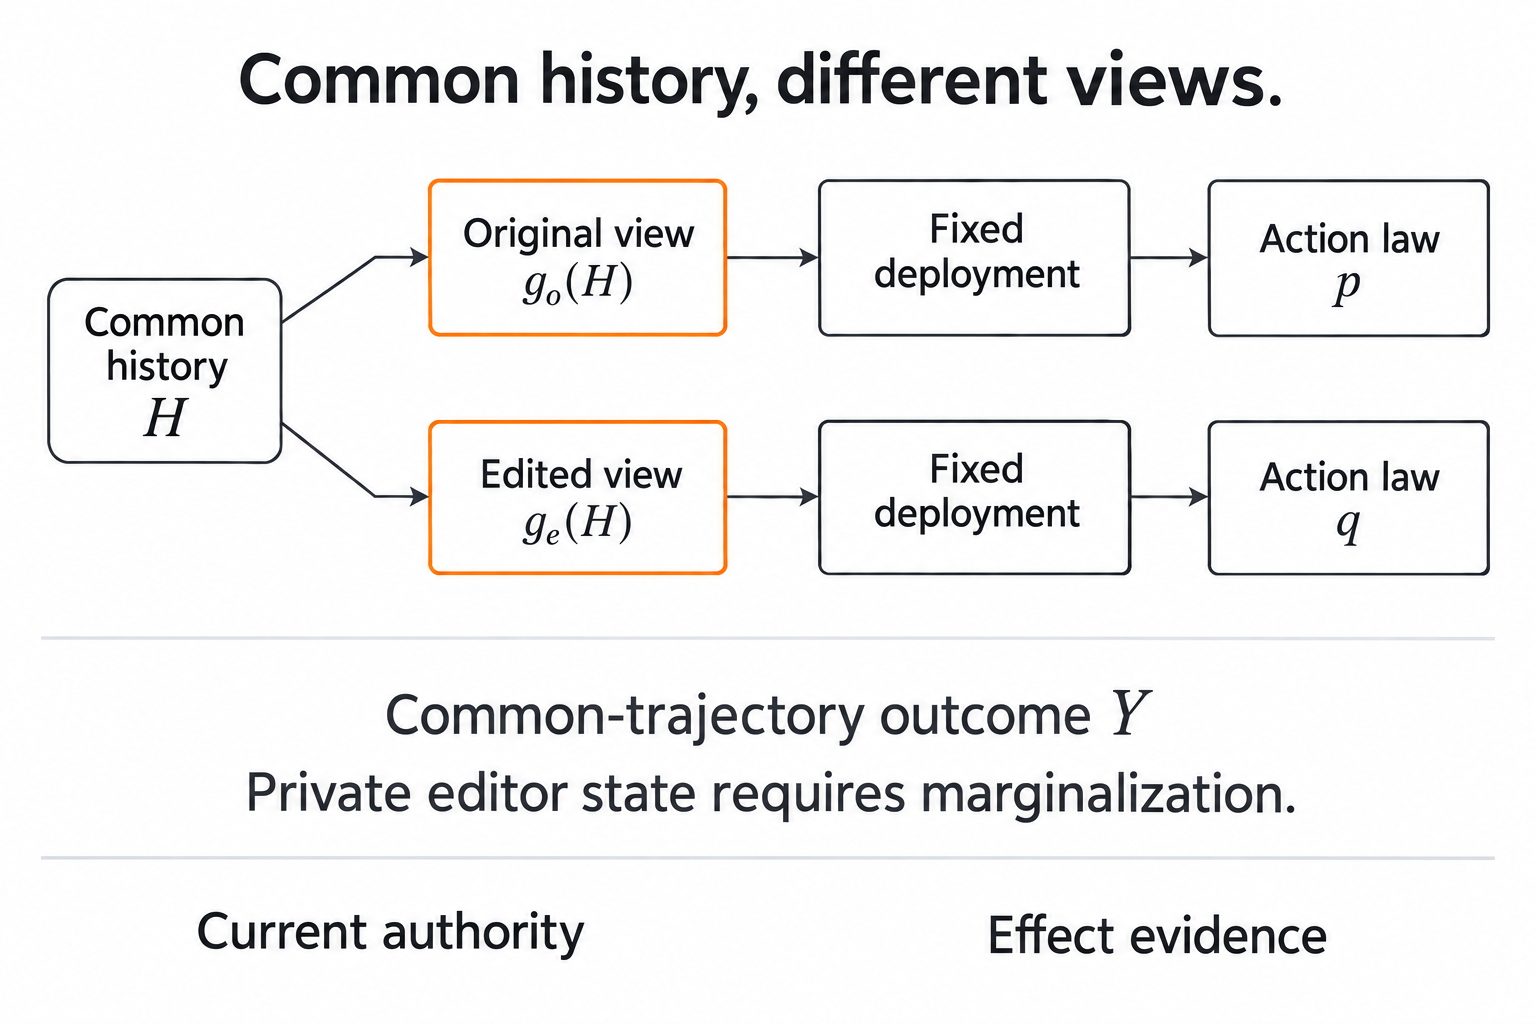
\includegraphics[width=\linewidth]{book/figures/assets/F17review.png}
\caption{Different deterministic views of common permitted recorded history $H$ can induce different action laws $p,q$ under one fixed deployment. Model/tokenizer, decoder, parser and decision interface are held fixed. The behavioral bound concerns outcomes $Y$ on the common trajectory; random private editor state requires conditional marginalization. Two sampled prompts do not establish that premise. Current authority and effect evidence remain independent checks.}
\label{fig:C17:overview}
\end{figure}

\section{The conditioning record is part of the data}\label{sec:C17:conditioning}
For a sampled token or action $y_t$, let $c_t^{b}$ be the actual behavior context and $q_t(y)=\pi_{\theta_b,\delta_b}(y\mid c_t^{b})$ its behavior distribution. A likelihood term interpreted as behavior replay requires the actual decoded conditional law and relevant record, not merely the final transcript. Token laws and parsed-action laws are different sample spaces, as established in Chapter~\ref{ch:C02}. Privileged teacher labels remain possible supervision, but are not exact replay probabilities. An edit at a later time can remove information that was present earlier; an append-only physical log can retain information that a later decision no longer saw. Either reconstruction can therefore be wrong for a particular target.

MemoryWalker identifies these two flattening failures and gives exact tree-consistent reconstructions plus an approximate distillation approach~\cite{j2026memorywalker}. The exact methods preserve the live conditioning path; their computational and masking requirements differ from ordinary single-sequence replay. Approximate alignment does not establish exact equivalence. The following analysis develops a general contract rather than reporting additional paper results.

Store a context-view identifier with each sampled span, together with its model, tokenizer, serialization, position treatment, and attention-mask version. The record should permit reconstruction of the exact visible prefix at that span's generation time. Recording only which raw messages existed is insufficient because an editor can select, reorder, summarize, or relabel them. Recording only the final visible messages is insufficient because later edits can change earlier conditioning retroactively in the reconstructed tape.

Consider an observation $o$ that is visible when action $a_1$ is sampled and evicted before action $a_2$. Training both actions on a final compressed history removes $o$ from $a_1$'s conditioning. Training both on the full physical log restores $o$ for $a_2$. The correct record has different views for the two actions. This example is a direct consequence of time-indexed conditioning; it does not depend on a particular model family or on whether the edited observation was useful.

An implementation can represent the views as immutable segments with references to shared prefixes, or as a tree with visibility masks. Storage deduplication can preserve shared content while retaining distinct conditioning paths. Numerical equivalence still requires an execution path that implements the intended positions and masks. A mask with the correct visible token set can be wrong if position identifiers differ from rollout, and a correct logical view can be wrong if a stale cache is reused.

The practical invariant is local and inspectable: every target interpreted as behavior replay should identify the conditional input and sampling law that generated it. Tests can compare replayed logits with recorded rollout logits under a frozen model, allowing for documented numerical differences. A small average discrepancy is a diagnostic, not a universal guarantee; rare large mismatches can dominate importance ratios or affect consequential actions.


\section{Likelihood ratios require support and the right history}\label{sec:C17:likelihood}
Suppose a target deployed policy $\pi_{\theta,\delta}$ is evaluated on actions sampled by $q$. At a fixed recorded information state $c_t$, a one-step importance ratio is
\begin{equation}
 w_t=\frac{\pi_{\theta,\delta}(a_t\mid c_t)}{q(a_t\mid c_t)}.
\end{equation}
The denominator is the probability under the actual sampling procedure, including temperature, truncation, and any constrained decoding. Recomputing a base-model softmax without those operations does not necessarily recover $q$. If behavior used a top-$k$ support restriction, the target must be absolutely continuous with respect to that support for unbiased off-policy reweighting over the same state distribution.

Changing $c_t$ is not an innocuous implementation shortcut. A denominator evaluated on a reconstructed context $\tilde c_t$ describes a different conditional experiment. Even if the model weights are identical, $\pi_{\theta_b,\delta_b}(a_t\mid\tilde c_t)$ need not equal the probability that generated $a_t$. A ratio formed with that value is not the original importance ratio. Clipping it can stabilize an optimizer while leaving the conditioning error conceptually unresolved.

For a full trajectory with fixed environment dynamics and compatible histories, the likelihood ratio includes a product of action-probability ratios. Long horizons can produce high variance because several modest deviations multiply. If memory or harness versions also differ, the trajectory law includes those transition policies as well. Reweighting only language-model tokens does not automatically correct a changed memory admission rule or a changed tool router. The estimated objective must identify which parts of the generative process are being corrected.

Make that boundary explicit by recording both a context-control action $u_t$ and a task action $a_t$. Let $s_t$ be the complete recorded information state before $u_t$; behavior uses $\mu_b(u_t\mid s_t)$ and $\pi_b(a_t\mid c_t)$, while the target uses $\mu(u_t\mid s_t)$ and $\pi(a_t\mid c_t)$. If both processes share the initial law, deterministic assembly $c_t=g(s_t,u_t)$, and environment transition kernel, then on common support
\begin{equation}
 \frac{dP_{\mu,\pi}}{dP_{\mu_b,\pi_b}}(\tau)
 =\prod_{t=0}^{T-1}
 \frac{\mu(u_t\mid s_t)}{\mu_b(u_t\mid s_t)}
 \frac{\pi(a_t\mid c_t)}{\pi_b(a_t\mid c_t)}.
\end{equation}
The common factors cancel; stochastic memory writes require additional factors unless their kernels are shared. An editor that deterministically retains a span in behavior but deterministically deletes it under the target can violate trajectory support. A token ratio computed after deletion does not create the missing editing transition. If assembly itself changes, it must be represented in the state or transition law rather than silently treated as the same $g$. This identifies exactly when an LM-only correction is incomplete without implying that an empirical approximation is unusable.

The support condition is particularly important after tool-schema changes. A new tool action may have zero probability under the old behavior policy because the tool did not exist or its arguments were forbidden. No finite weight can recover samples of that action from an old dataset. Additional exploration or a different estimand is required. Calling the update ``off-policy corrected'' does not remove missing support.

Privileged training information creates another boundary. A teacher can condition on a successful solution or an oracle skill that the deployed policy does not receive. Distillation can transfer useful behavior, but the training conditional is intentionally different. That should be described as teacher-guided learning, not exact replay of the deployment process. The question becomes whether the student generalizes under its actual information state, with contamination and privilege leakage controlled.

These are mathematical deductions from conditional probability and change of measure. They do not imply that every approximate training pipeline fails in practice. They identify what an exact claim would require and why empirical success alone does not validate an incorrect likelihood interpretation. The appropriate experiment records behavior probabilities, reconstructs views, checks support, and reports the sensitivity of outcomes to the approximation.

A numerical construction illustrates why the wrong history cannot be repaired by a ratio computed more precisely. Suppose a binary observation $o$ is equally likely to be zero or one. The behavior policy selects $a=1$ with probability $0.9$ when $o=1$ and $0.1$ when $o=0$. After the observation is removed, the marginal probability of $a=1$ is $0.5$. For a sampled pair with $o=1,a=1$, the actual denominator is $0.9$, not $0.5$. Using the marginal denominator inflates a target probability of $0.9$ from an exact ratio of one to a spurious ratio of $1.8$. No floating-point improvement fixes that conditioning substitution. These values define a hypothetical probability model; they are not measured model outputs.

If the target policy genuinely does not observe $o$, its numerator should use the target's restricted information state. The trajectory estimator must still account for how the data were collected and what quantity is being estimated. One cannot silently replace both numerator and denominator with a new marginal experiment and claim equivalence to the original conditional objective. The distinction is especially consequential when outcome or advantage estimates also depend on the missing observation.

The same construction can be implemented as a controlled rollout test with a visible bit, an edit, and a later tool decision. Record the generated action probability before editing, then compare replay under the live view, the final compacted view, and the full log. The expected ordering follows from the constructed distributions only if the model actually learns those distributions; an empirical study must measure rather than assume that condition. This separates a mathematical counterexample from a claim about how a particular language model behaves.


\section{A bounded behavior-preservation proposition}\label{sec:C17:bound}
Consider two finite-horizon agent variants on a common observation/action/environment trajectory space. Let $h_t$ be its history immediately before action $t$, excluding variant-private context, memory and editor metadata. Both variants have the same initial law and the same nonpolicy observation/environment kernels conditional on this history and action, and use a common complete action alphabet including failure or termination outcomes. The horizon is $T\in\mathbb N_{>0}$; terminated runs are padded by the same absorbing outcome. The laws $p_t(\cdot\mid h_t)$ and $q_t(\cdot\mid h_t)$ are the actual action distributions conditional on this common history. For deterministic context constructors they are obtained by applying each constructor and the deployed decoder to $h_t$. With random private editor state, they must instead marginalize its conditional law; a model distribution at one sampled prompt does not establish this premise. At every matched reachable history, assume $\operatorname{TV}(p_t,q_t)\leq\varepsilon_t$, where $0\leq\varepsilon_t\leq1$. Couple initial states identically and couple actions maximally while the common histories agree. Conditional on no earlier divergence, agreement at step $t$ has probability at least $1-\varepsilon_t$. Therefore, for the same $[0,1]$-valued functional $Y$ measurable on this common trajectory space,
\begin{equation}
 |\mathbb EY_{\rm orig}-\mathbb EY_{\rm edit}|
 \leq1-\prod_{t=0}^{T-1}(1-\varepsilon_t)
 \leq\min\!\left(1,\sum_{t=0}^{T-1}\varepsilon_t\right).
 \label{eq:C17:coupling}
\end{equation}
The first bound follows because identical trajectories have identical $Y$, while its difference is at most one after divergence. No independence of stepwise errors is assumed. For uniform $\varepsilon_t=\varepsilon$, the bound becomes $1-(1-\varepsilon)^T\leq\min(1,T\varepsilon)$. This is a standard coupling deduction under explicit hypotheses, not a measured guarantee for a context editor.

A KL premise permits a sharper horizon dependence than applying Pinsker separately at every step. Let $P$ and $Q$ be the laws of the common trajectory projection just defined, and require $P\ll Q$. With common nonpolicy factors, the chain rule gives
\begin{equation}
 \operatorname{KL}(P\Vert Q)=
 \sum_{t=0}^{T-1}\mathbb E_{h_t\sim P}
 \operatorname{KL}\{p_t(\cdot\mid h_t)\Vert q_t(\cdot\mid h_t)\}.
\end{equation}
Thus, if this sum is at most a finite $K_T\geq0$, the bounded-functional variational inequality and Pinsker's inequality yield
\begin{equation}
 |\mathbb EY_{\rm orig}-\mathbb EY_{\rm edit}|
 \leq\min(1,\sqrt{K_T/2}).
\end{equation}
Natural logarithms and $\operatorname{TV}=\sup_B|P(B)-Q(B)|$ are used~\cite{ch02_reid2011}. A uniform conditional KL bound $\eta$ implies $K_T\leq T\eta$, giving $\min(1,\sqrt{T\eta/2})$. The stronger population premise can also hold as an expectation under the original trajectory distribution without being uniform. A finite average over unrelated ordinary prompts establishes neither premise. Estimating the relevant expectation still needs the sampling and uncertainty controls of Chapter~\ref{ch:C02}; rare missing obligations can remain untested.

The histories in these comparisons are matched common histories, even though each variant constructs a different model-visible view from them. The result bounds observable task outcomes on this projection. It does not bound functionals of private memory, context strings or internal metadata: those can differ even when every action agrees. Enlarging the trajectory to include such variables requires their transition kernels in the likelihood ratio and coupling. Changing environment dynamics, tool effects or authorization kernels likewise invalidates cancellation unless those changes are modeled. Once coupled trajectories diverge, later inputs may differ arbitrarily; the coupling bound does not assume they remain close. A cumulative reward requires its own bounded range rather than silently reusing the terminal $[0,1]$ scale.

There is a separate exact enforcement property. If a trusted monitor admits only actions in its current allowed set and mediates every consequential effect, a context edit cannot dispatch an outside action through that monitor. The property depends on correct interpretation, current authority and complete mediation; it still permits allowed but wrong actions. It does not establish effect-ledger truth or task correctness. This keeps the proposal, authority and recorded-effect contracts separate.

For a falsifiable experiment, freeze the decoder, parser, tools, environment fixture and current authority, then compare next-action laws at matched pre-edit states. Report the worst observed cases, missing support, and the workload sampling distribution. Neither an empirical maximum nor a few repeated continuations establishes a global supremum over histories. The derivations identify what must be bounded; they do not supply the required evidence by themselves.

\section{Memory transactions and semantic validity}\label{sec:C17:transactions}
Transactional consistency preserves relationships among reads and writes; semantic validity concerns whether the recorded assertions and procedures are appropriate. A database can provide atomic updates that commit a false summary perfectly. A language model can produce an accurate summary whose references become inconsistent because another writer changes the source before commit. An agent memory system needs both a storage contract and a semantic admission contract.

Let a proposed update read objects $R$ at versions $v_R$ and produce writes $W$. An optimistic commit validates that the relevant read versions still match. If not, the update should be recomputed, merged under a justified rule, or rejected. The hard part is identifying the relevant read set. Generated abstractions can depend on a source that was seen earlier but omitted from the recorded extraction input. Missing provenance defeats conflict detection even if the database transaction implementation is correct.

The RecMem consolidation path in Chapter~\ref{ch:C14} illustrates a multi-layer publication boundary: episodes, semantic facts, and raw-memory deletion are distinct operations~\cite{repo_recmem2026}. HyperSkill maintenance similarly changes nodes, embeddings, and membership relations~\cite{repo_hyperskill2026}. A partially persisted update can make one representation disagree with another. The required invariant is not simply ``all writes completed,'' but that every published object has valid dependencies and can be interpreted under the same versioned schema.

Semantic validity needs richer conflict classes. A later observation can supersede a current fact without invalidating the truth of its historical episode. A skill can become incompatible with a new tool while remaining an accurate record of a past successful procedure. An authorization can expire without deleting the evidence that it once existed. These cases require status transitions, not indiscriminate overwrite or deletion.

Linearizable memory operations can support reasoning about a single shared object's update order~\cite{herlihy1990linearizability}. They do not determine whether the chosen semantic resolver is correct. A last-write-wins fact register can be linearizable while choosing the wrong assertion because the later writer had lower authority or described an older valid-time interval. Storage guarantees should therefore be stated using the actual abstract data type and application semantics.

A proposed semantic transaction writes candidate assertions with source links, validates role and authority, resolves temporal status, and atomically publishes a coherent view. If validation is model-based, retain its uncertainty and evidence rather than calling the transaction verified in the formal sense. For high-consequence obligations, deterministic fields can constrain what the model may revise. The goal is not to make every memory fact formally provable, but to prevent unexamined semantic changes from masquerading as ordinary storage maintenance.


\section{Model index and tool migration}\label{sec:C17:migration}
Memory portability depends on the consumer. A concise skill written for one model can rely on its implicit knowledge or compensate for its characteristic mistakes. A new model may interpret the same text differently. A new embedding model can change the geometry of queries and records. A new tool schema can invalidate a previously successful procedure. Version identifiers make these changes visible but do not establish compatibility.

An embedding example makes the issue precise. Suppose document vectors $d$ and queries $q$ originally share a space with score $q^{\mathsf T}d$. A replacement encoder applies an orthogonal rotation $R$ to both, preserving within-space dot products. If only queries are updated, the score becomes $(Rq)^{\mathsf T}d$, which generally differs from $q^{\mathsf T}d$. Even an information-preserving coordinate change breaks mixed-version retrieval. Re-embedding both sides or using a validated alignment is required. This is a mathematical example, not a benchmark result about named embeddings.

For policy migration, preserve the old memory snapshot and compare the new model on matched tasks with no memory, original memory, and a revised memory representation. This separates backbone changes from memory compatibility. Include cases where the old memory should be ignored. A new model that applies every old instruction more aggressively can improve some recall tasks while violating current constraints. Positive transfer and overuse need separate outcomes.

Tool migration can be more discrete. Changing an argument's default, resource scope, or side-effect semantics can invalidate a skill even when its function name remains unchanged. Attach schema and behavior versions to the skill's compatibility record, and require fresh validation when relevant contracts change. A schema-compatible change can still alter semantics; syntactic validation is necessary but insufficient.

CLM's inspected environment shows a useful local boundary: \texttt{ContextEnv.step} writes the live mirror, executes a command, reads the mirror back, and applies a parsed edit through \path{_apply_edit}. The edit gate checks growth against a configured rule, and the parser retains a protected prefix~\cite{repo_clm2026}. This validates some structural and budget conditions, not the truth of every rewritten assertion. Migrating that environment to a new tokenizer or parser changes what the gate counts and which messages it reconstructs.

A successful edit is also not synonymous with fitting the token budget. In the inspected \path{_apply_edit} branch, growth is subject to the configured growth/fit rule, but a shrinking edit can be applied while the result remains over the limit; the readout then requests further compaction~\cite{repo_clm2026}. The synchronization counter likewise does not prove behavioral preservation. An integration should record applied versus rejected edits, final enforced token counts, and the actual next-decision input separately. Structural acceptance supplies no bound on $\mathsf P_\epsilon$.

A migration gate should therefore cover the entire path from stored record to dispatched effect. Record old and new versions, representative compatibility tests, unresolved failures, and rollback criteria. If a proprietary model version cannot be pinned exactly, state that reproducibility limit and use dated API identifiers and observed behavior. A rolling service name is not a reproducible policy identity.

The October 2026 skill--policy co-evolution study makes this dependence experimentally explicit through CODA. It perturbs the delivered skill bank and evaluates consistency under meaning-preserving rewrites, resistance to corrupted guidance, and worst-case success~\cite{feng2026coda}. Its theory concerns candidate coverage and a specified cooperative acceptance rule, not every conceivable self-improvement objective. Its stress-test losses also do not estimate how frequently equivalent drift occurs in deployment. The result is a concrete warning against evaluating only the policy-bank pair that was selected together.

A corresponding original diagnosis separates three perturbations. Rewrite surface form while preserving procedural meaning, alter valid preconditions while retaining familiar wording, and replace the consumer policy while freezing the bank. The first tests interpretive invariance, the second tests applicability sensitivity, and the third tests portability. Pooling them into one robustness number can reward the wrong behavior: a policy should ignore irrelevant wording changes but respond to a changed precondition. Consistency is therefore invariance to specified transformations and sensitivity to others, not indiscriminate resistance to change.


\section{Authority must survive every transformation}\label{sec:C17:authority}
Authority is information about who may direct which effects under what conditions. It should not be inferred from memory frequency, semantic relevance, or the confidence of a generated summary. A retrieved page can be highly relevant to a task while being untrusted as an instruction source. A stored skill can be useful while lacking authority to change the task. A prior session can contain valid historical permission that no longer applies.

Progent represents allowed tool calls through symbolic policies and distinguishes narrowing from expansion~\cite{corpus250411703}. Under complete mediation, an unapproved update can be restricted to a subset of the previous allowed set. Write this as $\mathcal A_{t+1}\subseteq\mathcal A_t$ for automatically accepted narrowing. The comparison must use the same current authority epoch; an allowed set restored from an old snapshot is not the current grant. The guarantee depends on correct policy interpretation, a trusted enforcement boundary, and every consequential call passing through it. It does not guarantee that all allowed calls are useful or semantically correct.

Compaction can preserve authority in two ways. It can retain the original authoritative statement verbatim, or it can preserve a validated typed representation whose semantics are enforced independently. A generated paraphrase without validation can weaken or broaden a condition. For example, ``prepare a draft for review'' can become ``complete the publication task'' after repeated summarization. The model may then believe a broader objective even if the external monitor still blocks publishing. Preserving both behavioral guidance and enforcement reduces this mismatch.

Concurrent updates create races. A worker may choose an action under authority version $a$ while a user narrows scope to $a+1$. Checking permission only at worker creation is insufficient if the effect occurs later. The dispatcher should evaluate the current applicable policy or require a validated authorization lease whose semantics cover that interval. Canceling the worker is not equivalent to preventing an already dispatched effect.

The proposed test records authority at task creation, context assembly, action proposal, and effect dispatch. Inject a narrowing correction between each pair of stages. Check whether stale proposals are rejected and whether the user-visible state accurately reports any in-flight uncertainty. This targets authority consistency directly instead of relying on a general prompt-injection benchmark to discover the race accidentally.

Authority preservation also constrains learning. A memory writer should not turn a successful prohibited action into a reusable recommendation merely because the environment rewarded it. Outcome feedback and authorization are separate channels. A system can perform well on a task-success metric while learning procedures that violate its intended scope. The evaluation must retain both dimensions and report their interaction.


\section{A consistency audit with causal counterexamples}\label{sec:C17:audit}
A proposed audit begins with a versioned dependency manifest for each consequential decision. It records the active context, memory snapshot, retrieved evidence, policy configuration, tool schema, authority, and relevant environment observations. The manifest is not a claim of full observability. It states which dependencies are known and makes missing dependencies visible. A reconstruction that silently substitutes current versions defeats the purpose.

The first test class targets conditioning: restore the same frozen model and compare the recorded live input with training reconstruction. The second targets semantic updates: create near-identical records with different valid times or authority and inspect whether consolidation preserves the distinction. The third targets migration: update only the query encoder, tool schema, or model consumer and measure compatibility failures. The fourth targets concurrency and effect timing. These tests exercise different consistency properties and should retain separate results.

Counterexamples should be minimal enough to identify the missing contract. If a summary loses a publication restriction, the failure record includes the source restriction, summary, action proposal, and monitor outcome. If an index returns a stale passage, preserve the source version and embedding generation. If a skill overgeneralizes after a model upgrade, compare its applicability and execution under both consumers. A final wrong answer alone does not identify which transition failed.

Causal attribution requires controlled substitutions. Change one component at a time where feasible, but acknowledge interactions. A new model may need a different prompt format, making a literal prompt hold-fixed comparison unrepresentative. In that case report both a strict component substitution and an adapted configuration, charging the adaptation effort separately. This avoids treating either one comparison as the only legitimate view.

No new audit outcomes are claimed here. The propositions and protocols are deductions and proposed experiments grounded in the mechanisms reviewed. Their purpose is to turn vague continuity claims into explicit conditions that can fail. A coherent agent architecture should be able to state which transitions are exact, which are approximate, which depend on model judgment, and which are unknown.

The cross-layer conclusion is that context, memory, and policy must evolve under compatible contracts. More storage does not repair wrong conditioning; correct transactions do not make a false abstraction true; a current model does not make old skills compatible; and a well-formed tool call does not establish authorization. Treating these distinctions together provides a technical basis for reliable stateful execution without claiming a general solution to intelligence.

